\documentclass[emulatestandardclasses]{scrartcl}
\usepackage{graphicx}
\usepackage{color}
\usepackage[ngerman]{babel}
\usepackage{hyperref}
\usepackage{fullpage}
\usepackage[utf8]{inputenc}
\usepackage{calc} 
\usepackage{enumitem}
\usepackage{titlesec}
\newcommand{\todo}[1]{\textcolor{red}{TODO: #1}\PackageWarning{TODO:}{#1!}}
\date{\vspace{-3ex}}
\begin{document}

\title{
	\includegraphics*[width=0.75\textwidth]{ErstesSem/images/hu_logo.png}\\
	\vspace{24pt}
	Plato's Phaedo}
\subtitle{\vspace{10pt}Proseminar WS 17/18\\
          David Ebrey\\
          Philosophisches Institut I \\ 
          Humboldt Universit"at zu Berlin}
\author{Lennard Wolf\\
        \small{\href{mailto:lennard.wolf@student.hu-berlin.de}{lennard.wolf@student.hu-berlin.de}}}
\maketitle
\begin{abstract}
In this seminar we will carefully work through Plato's Phaedo, which discusses ethical, epistemological, and metaphysical ideas that at the heart of Plato’s philosophy. Topics covered include: causation, the nature of the soul, the problems caused by the body, how inquiry is possible, the proper attitude and methodology for inquiry, why (and in what sense) the forms are distinct from sensible things, and why the best life is spent contemplating the forms. We will also discuss how the literary elements of the dialogue are related to its philosophical ideas.
The seminar will be in English and will assume basic familiarity with Plato's works. Knowledge of Greek is not required, but we will occasionally discuss the Greek, as needed.
\end{abstract}
\newpage

\tableofcontents
%\listoffigures
\newpage


\section{Introduction\\(19.10.17)}

\begin{itemize}
  \item Reading: Phaedo until next week
  \item Should read Laches before!
  \item Ecthyphro would be good 
  \item laches authyphro cooper
  \item Apology!!
  \item every week one page assignment to write what is confusing you?
  \item 15 to 20 pages! during the semester meeting! what is the central question to answer in the paper? how to go about it? hand in draft by March 15!
  \item apology, laches, phaedo 
\end{itemize}


\subsection{}

\begin{itemize}
  \item The early/Socratic dialogues: Laches, Euthyphro, Apology
  \item "`Unfolding Struucture"' of the dialogue: some claims are explained later in the text, but not explicitly!
  \item What is it? $\rightarrow$ "`Form"'
  \item  
\end{itemize}


\newpage
%\section{"Uber den Professor}
%Matthias Schlo"sberger ist Heisenbergstipendiat der Deutschen Forschungsgemeinschaft
%an der Humboldt Universit"at zu Berlin mit dem Forschungsprojekt "`Die Erfahrung der Realit"at durch Widerstand"'.
%
%\begin{figure}[h]
%	\centering
%	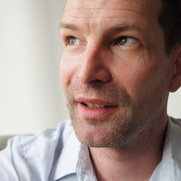
\includegraphics[width=0.3\textwidth]{images/Matthias_Schlossberger.png}
%	\caption{Matthias Schlo"sberger}
%	\label{fig:MS}
%\end{figure}


%\begin{figure}[h]
%	\centering
%	
\includegraphics[width=0.5\textwidth]{images/template.png}
%	\caption{Template Bild}
%	\label{fig:template}
%\end{figure}

\end{document}
